\documentclass[a4paper,twoside]{iiththesis}
\usepackage{graphicx}
\usepackage{caption} 
\captionsetup[table]{skip=10pt}
\usepackage{lscape}
\usepackage{float}
\usepackage{tcolorbox}
\usepackage{hyperref}
\book{Thesis Stage II }
\title{Intelligent Drone for Detecting Real-time Object using Machine Learning and Artificial Intelligence}
\degree{M.Tech. in Smart Mobility}
\department{Smart Mobility (Interdisciplinary)}
\submitted{June 2022}
\author{Abhishek Kumar}
\adviser{Dr. G V V Sharma}
\addradviser{Dept. of Electrical Engineering\\ IIT Hyderabad}
%\chair{---------}
%\addrchair{Dept. of Mech Eng \\ IITH}
%\external{----------}
%\addrexternal{Dept. of Chem Eng \\ IITM}
%\internal{----------}
%\addrinternal{Dept. Math \\ IITH}
%\coguide{----------}
%\addrcoguide{Dept. of Chem Eng \\ IITH}
\abstract{
\par This thesis is intended to serve as a concise and to-the-point report of my work in the domain of autonomous navigation of UGVs (Unmanned Ground Vehicles) and UAVs (Unmanned Aerial Vehicles). A driver or operator is generally required to operate a ground vehicle (car, bus, etc.) or an aerial vehicle (quad-copter, etc.). These operators/drivers must be trained, and obtaining a license is also a tedious process (especially for aerial vehicles). In reality, these factors prevent us from utilizing these machines to their full potential and exploring their wide array of valuable applications.
\par By automating ground vehicles, we could save on fuel, reduce accident-related costs, and improve overall transportation efficiency. An autonomous aerial vehicle, on the other hand, can be used for many purposes, including: Food and medical delivery in remote areas, Public safety in calamities, Bridge and power lines inspection, Agriculture, Road accident report, Traffic monitoring, and Transportation.

}
\acknowledgements{.}
\dedication{.}


\renewcommand{\bibname}{References}
\begin{document}


\chapter{Introduction}
\section{Micro-Controllers and their specifications}
\subsection{Raspberry Pi 3B}
\par  Raspberry Pi (RPi) is an on-board computer and it is among the most popular development boards. The Raspberry Pi runs a customized version of Linux called Raspberry Pi OS. It has all the features of a personal computer. This board has USB interfaces that allow it to connect to peripherals (such as a mouse and keyboard), USB storage, etc. HDMI interface can be used to connect displays to the board having up to 4K resolution. Additionally, it has other ports/interfaces, including USB-C (power), a 2-lane MIPI CSI port (camera), a 3.5mm audio jack (audio), and RJ-45 (Ethernet). WiFi and Bluetooth 5.0 support are provided by the Raspberry Pi.
\subsection{ESP32} 
\par  ESP32 is a family of low cost and low power system on a chip (SoC) micro-controllers. It is enabled with dual mode bluetooth and integrated Wi-Fi.It is a successor to the ESP8266 micro-controller. Tensilica Xtensa 32-bit LX6 is main processor inside ESP32. It has memory of 320 KiB RAM and 448 KiB ROM. It contains 34 programmable GPOIs, 12-bit SAR ADC up to 18 channels, two 8-bit DACs, four SPI, two I2S and I2C and three UART interfaces.I have used ESP32-WROOM-32 module for my projects.

\begin{table}[H]
\centering

\begin{tabular}{|l|c|c|c|}
\hline
\textbf{Parameters} & \textbf{Raspberry Pi 3B} & \textbf{ESP-32} \\ \hline
\textbf{Processor} & \begin{tabular}[c]{@{}c@{}}Quad-core Broadcom \\ BCM2837 (4×Cortex-A53)\end{tabular} & \begin{tabular}[c]{@{}c@{}}Xtensa Dual-Core 32-bit \\ LX6 with 600 DMIPS\end{tabular} \\ \hline
\textbf{GPU} & \begin{tabular}[c]{@{}c@{}}Broadcom VideoCore IV \\ @ 250 MHz\end{tabular} & - \\ \hline
\textbf{Operating voltage} & 5V & 3.3V \\ \hline
\textbf{Clock speed} & 1.2GHz & 26 MHz – 52 MHz \\ \hline
\textbf{System memory} & 1 GB & \textless{}45kB \\ \hline
\textbf{Flash memory} & - & up to 128MB \\ \hline
\textbf{EEPROM}  & - & - \\ \hline
\textbf{\begin{tabular}[c]{@{}l@{}}Communication \\ supported\end{tabular}} & \begin{tabular}[c]{@{}c@{}}IEEE 802.11 b/g/n\\ Bluetooth, Ethernet Serial\end{tabular} & IEEE 802.11 b/g/n \\ \hline
\textbf{\begin{tabular}[c]{@{}l@{}}Development \\ environments\end{tabular}} & \begin{tabular}[c]{@{}c@{}}Any linux \\ compatible IDE\end{tabular} & Arduino IDE, Lua Loader \\ \hline
\textbf{\begin{tabular}[c]{@{}l@{}}Programming \\ language\end{tabular}} & \begin{tabular}[c]{@{}c@{}}Python, C, C++, Java,\\ Scratch, Ruby\end{tabular} & Embedded C, C++ \\ \hline
\textbf{I/O Connectivity} & \begin{tabular}[c]{@{}c@{}}SPI DSI UART \\ SDIOCSI GPIO\end{tabular} & UART, GPIO \\ \hline
\end{tabular}
\caption{Comparison between Raspberry Pi 3B and ESP-32}
\end{table}

%



\chapter{UAV (Unmanned Aerial Vehicle)}
\section{Quad-copter (Drone)}
\subsection{Introduction} 
\par  Innovative work on unmanned aerial vehicles (UAVs) is getting high consolation these days, since the applications of UAV can apply to many areas such as military, salvage mission, film making, farming, and others.
In remote areas like border areas or agricultural fields to monitor the situations on a daily basis, for surveillance in those areas, Unmanned Aerial Vehicle(UAV) plays an important role. UAV is also known as Drone and has a lot of attention nowadays. Drones are generally used at the border areas which cannot be done manually by military forces.
The quad-copter works according to the force or thrust generated by four rotors connected to its body. It has four input and six yield or output states (x, y, z, θ, ψ, ω), and it is an under-activated framework, since this empowers quad-copter has to convey more load.
\subsection{Quad-copter Motion Mechanism}
\par Quad-copter can be described as a vehicle with four propellers joined to the rotor found at the cross casing. This goes for altered pitch rotors driven to control the vehicle movement. The velocities of these four rotors are independent. By controlling the pitch, roll and yaw angle, the position of the vehicle can be controlled effectively.
\par Quad-copter has four inputs, and essentially the thrust is generated by the propellers attached to the rotors. The speed of each motor is controlled independently, and the motion or direction of the quad-copter is controlled by varying the speed and direction of each motor.
-------------------------
\begin{figure}[h!]
\caption{Pitch direction of quad-copter}
\label{Pitch direction of quadcopter}
\centering
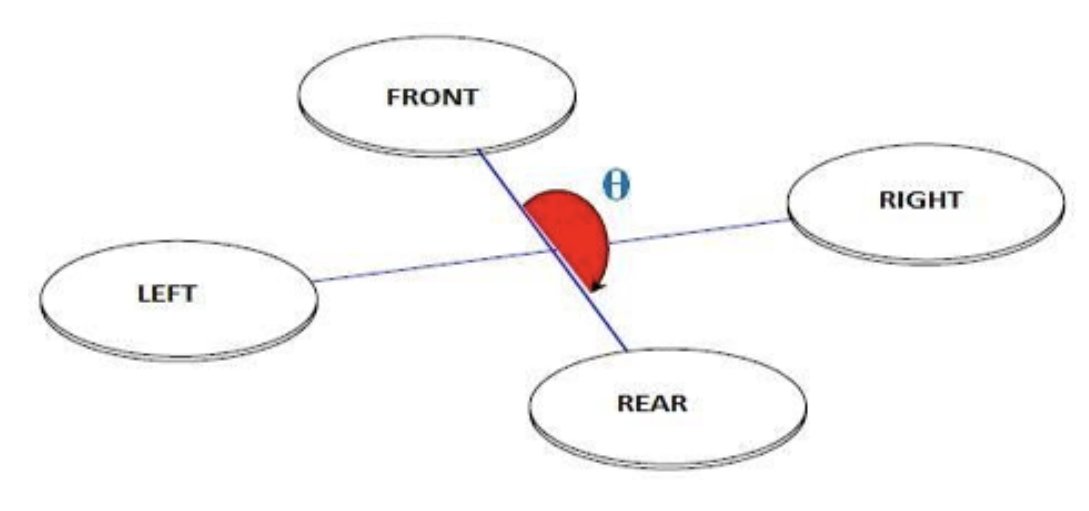
\includegraphics[width=\columnwidth]{./Figures/pitch_direction.png}
\end{figure}

\begin{figure}[h!]
\caption{Roll direction of quad-copter}
\label{Roll direction of quadcopter}
\centering
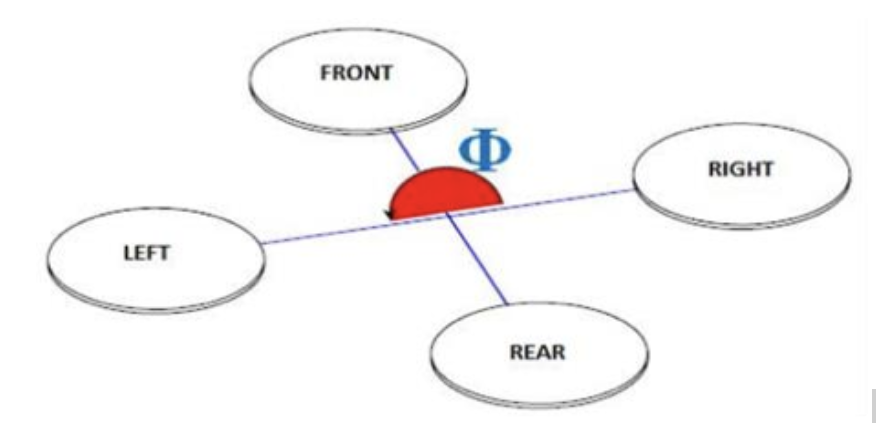
\includegraphics[width=\columnwidth]{./Figures/roll_direction.png}
\end{figure}

\begin{figure}[h!]
\caption{Yaw direction of quad-copter}
\label{Yaw direction of quadcopter}
\centering
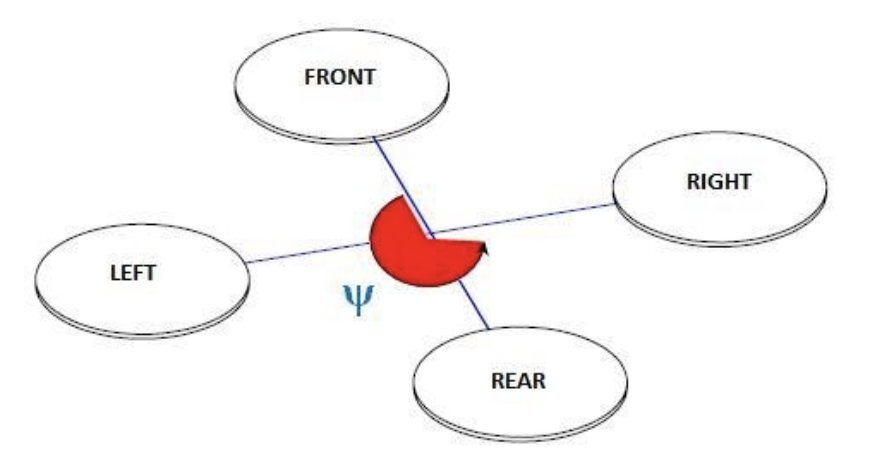
\includegraphics[width=\columnwidth]{./Figures/yaw_dir_qc.png}
\end{figure}

\subsection{Take-off and Landing Motion Mechanism}
\par Take-off motion is the motion that lifts the quad-copter from ground to hover position. As shown in Fig.4 there are a total four motors, two rotating in the clockwise direction and two rotating in counter clockwise direction. To fly the quad-copter in hover position, increase the speed of each rotor simultaneously. For landing the quad-copter to ground decrease the speed of each rotor simultaneously as shown in Fig. 5.

\begin{figure}[h!]
\caption{Take-off motion}
\label{Take-off motion}
\centering
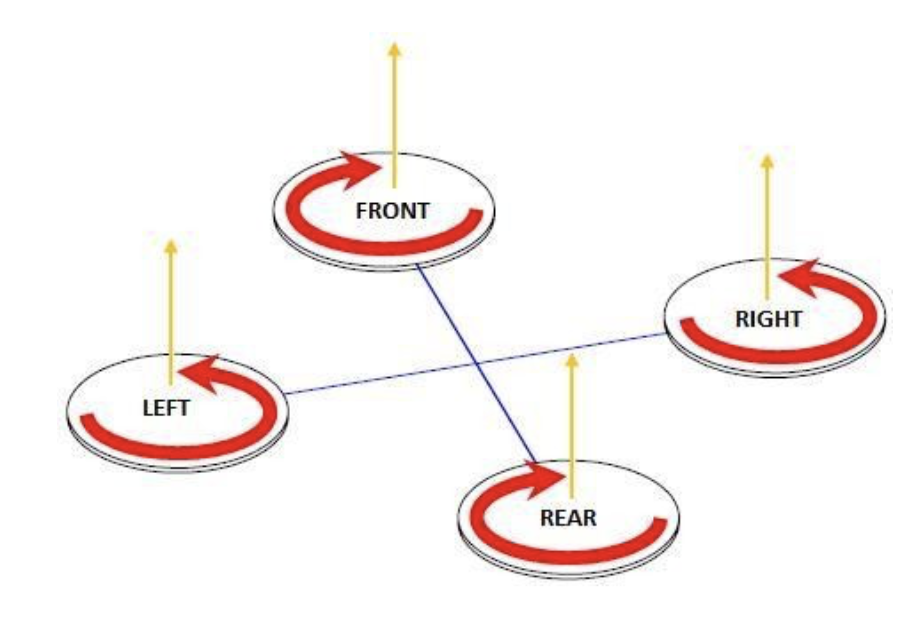
\includegraphics[width=\columnwidth]{./Figures/takeoff_qc.png}
\end{figure}

\begin{figure}[h!]
\caption{Landing Motion}
\label{Landing Motion}
\centering
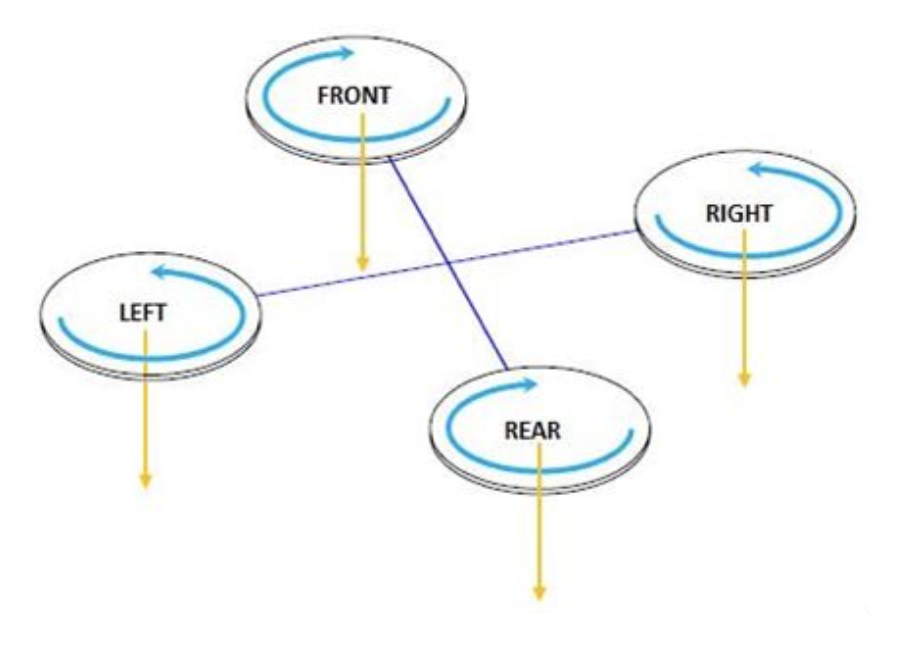
\includegraphics[width=\columnwidth]{./Figures/landing_motion_qc.png}
\end{figure}

\subsection{Forward and Backward Motion Mechanism}
\par Forward motion of the quad-copter is controlled by increasing the speed of the rear rotor and decreasing the speed of the front rotor simultaneously as shown in Fig. 6. Backward motion of the quad-copter is controlled by increasing the speed of the front rotor and decreasing the speed of the rear rotor simultaneously as shown in Fig. 7. Reducing the rear rotor speed and increasing the front rotor speed simultaneously will affect the pitch angle of the quad-copter.

\begin{figure}[h!]
\caption{Forward motion}
\label{Forward motion}
\centering
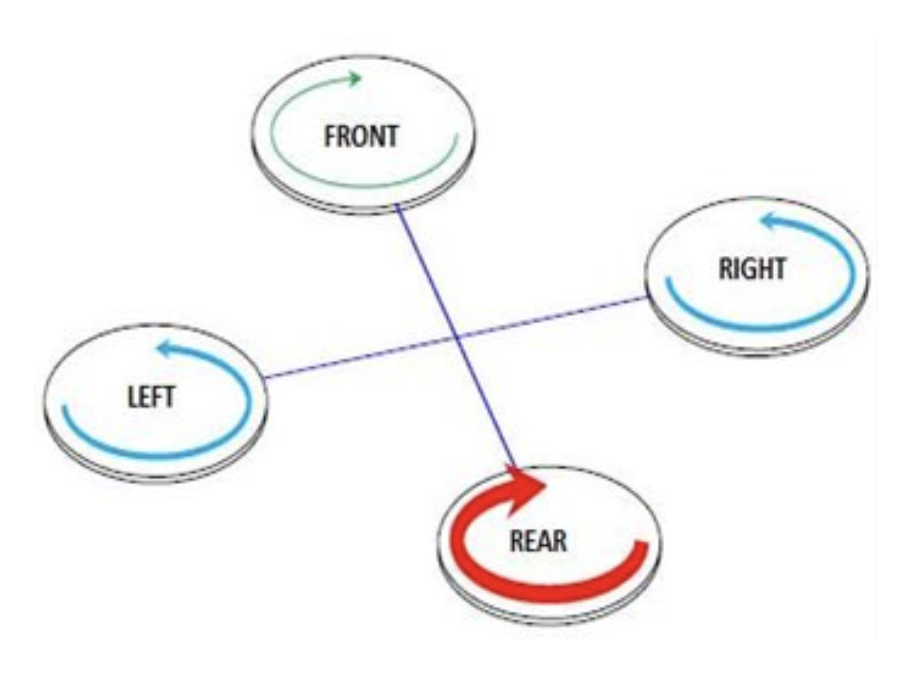
\includegraphics[width=\columnwidth]{./Figures/forward_motion_qc.png}
\end{figure}

\begin{figure}[h!]
\caption{Backward motion}
\label{Backward motion}
\centering
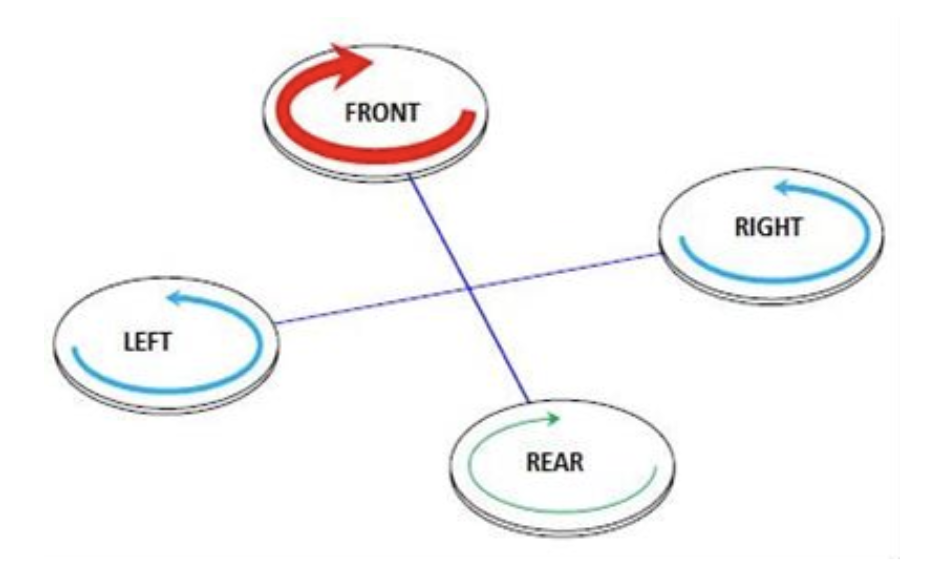
\includegraphics[width=\columnwidth]{./Figures/backward_motion_qc.png}
\end{figure}

\subsection{Left and Right Motion Mechanism}
\par The left and right motions of the quad-copter are controlled by changing the yaw angle. By increasing the speed of the counter-clockwise rotor and decreasing the speed of the clockwise rotor simultaneously, the quad-copter moves to the left side as shown in Fig. 8. Similarly by increasing the speed of the clockwise rotor and decreasing the speed of the counter-clockwise rotor simultaneously, the quad-copter moves to the right side as shown in Fig. 9.

\begin{figure}[h!]
\caption{Left and right motion}
\label{Left and right motion}
\centering
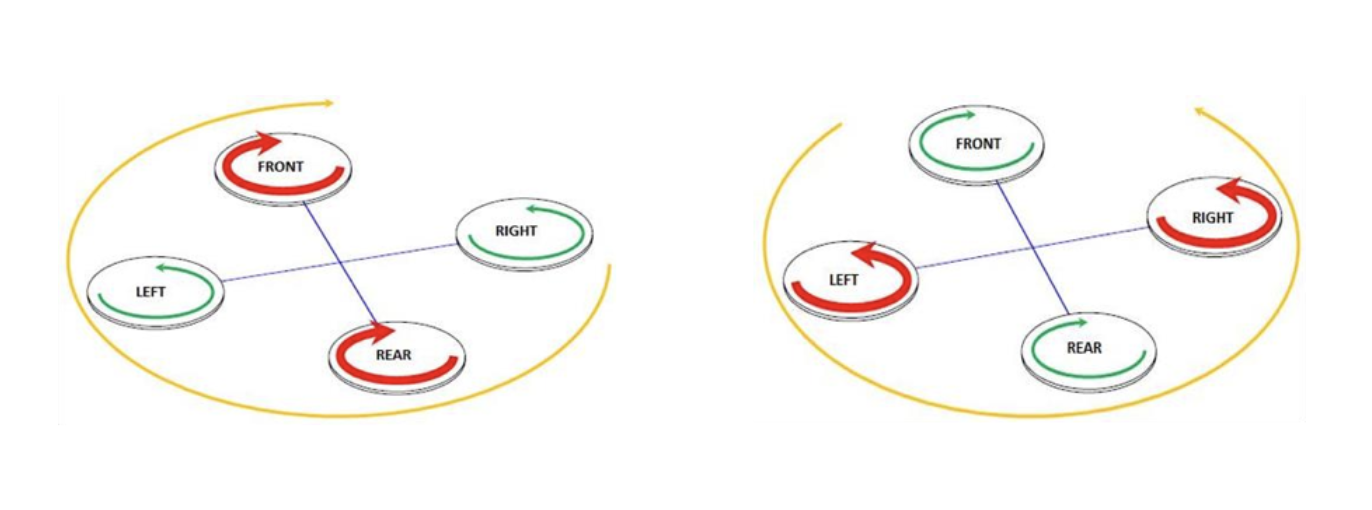
\includegraphics[width=\columnwidth]{./Figures/left_ryt_motion_qc.png}
\end{figure}

\subsection{Hovering and Static Position}
\par When two pairs of counter-clockwise and clockwise rotors rotate at the same speed, the quad-copter moves to hover position. At that time, the total addition of reaction torque is zero which allows the quad-copter to achieve hover position.


\subsection{Hardware requirements}
\begin{table}
\centering
\begin{tabular}{|l|l|l|} 
\hline
\textbf{Description}               & \textbf{Make~} & \textbf{Model}       \\ 
\hline
Frame(Quad-copter 4 axis)          & -              & F450                 \\ 
\hline
Motor (1000Kv)                     & -              & A2212/13T            \\ 
\hline
ESC (30 Amp)                       & Simonk         & 30A                  \\ 
\hline
APM Controller (2.8)               & ArduPilot      & APM 2.8              \\ 
\hline
Transmitters and Receiver~         & Flysky~        & Fs-i6 2.4Ghz         \\ 
\hline
Duracell Batteries for Transmitter & Duracell       & Ultra (Alkaline AA)  \\ 
\hline
GPS                                & Ublox~         & NEO 5 pin            \\ 
\hline
Battery~ (2200mAh 3S, ,11V)        & Shang yi       & B3 - 2200 mAH        \\ 
\hline
Battery Chargers (B3)              & imaxRC         & B3 pro~              \\ 
\hline
Propellers~ pairs (CW and ACW)     & -              & (10*4.5inch)         \\
\hline
\end{tabular}
\end{table}




\subsubsection{{Code link}}\label{Code_link_UGV_phone}
\begin{tcolorbox}
\url{https://github.com/sachinomdubey/Projects/tree/main/Autonomous\%20Navigation/UGV/ESP32/IDE/UGV_navigation_using_android_phone/Codes}
\end{tcolorbox}

% \begin{figure}[h!]
% \caption{Wiring Diagram for UGV Navigation using Android phone}
% \label{Wiring_UGV_phone}
% \centering
% \includegraphics[width=\columnwidth]{./Figures/Wiring_UGV_phone.png}
% \end{figure}

% \begin{figure}[h!]
% \caption{Flow Diagram for UGV Navigation using Android phone}
% \label{Flow_UGV_flysky}
% \centering
% \includegraphics[width=\columnwidth]{./Figures/Flow_UGV_phone.png}
% \end{figure}

% \subsubsection{Working}
% \begin{itemize}
%     \item User gives navigation input using the dabble app installed on the android device. The dabble app communicates to ESP32 over bluetooth. The dabble app UI is as shown in figure \ref{Dabble_app_UI}.
    
%     \begin{figure}[h!]
%     \caption{Dabble app user interface}
%     \label{Dabble_app_UI}
%     \centering
%     \includegraphics[width=12cm]{./Figures/Dabble_app_UI.jpg}
%     \end{figure}
%     \item Depending on the input received over bluetooth, the program sends suitable commands (forward, backward, left, right and stop) to the direction control pins of Motor driver IC.
% \end{itemize}

% \subsection{Navigation using Speech commands} 
% \subsubsection{Required components/Software tools}
% \begin{itemize}
%     \item  UGV chassis with DC motors
%     \item  ESP32 micro-controller with Type-B USB cable
%     \item  L293D Motor Driver IC
%     \item  Breadboard
%     \item  Jumper Wires
%     \item  Arduino IDE installed on system
%     \item Android Phone
% \end{itemize}



% \subsubsection{Steps}
% \begin{itemize}
%     \item Make the connections as per the wiring diagram (Figure \ref{Wiring_UGV_speech}).
%     \item Go to Arduino IDE and write the following program available on the \hyperlink{Code_link_UGV_speech}{code link}.
%     \item Compile and upload the program to ESP32 micro-controller using the Type-C programmable cable. 
%     \item Test whether the UGV is navigating as per the Speech command sent from the Android phone.
% \end{itemize}

% \subsubsection{\hypertarget{Code_link_UGV_speech}{Code link}}
% \begin{tcolorbox}
% \url{https://github.com/sachinomdubey/Projects/tree/main/Autonomous\%20Navigation/UGV/ESP32/IDE/Voice_Controll_UGV}
% \end{tcolorbox}

% \begin{figure}[h!]
% \caption{Wiring Diagram for UGV Navigation using Speech commands}
% \label{Wiring_UGV_speech}
% \centering
% \includegraphics[width=\columnwidth]{./Figures/Wiring_UGV_speech.png}
% \end{figure}

% \begin{figure}[h!]
% \caption{Flow Diagram for UGV Navigation using Speech commands}
% \label{Flow_UGV_speech}
% \centering
% \includegraphics[width=\columnwidth]{./Figures/Flow_UGV_speech.png}
% \end{figure}

% \subsubsection{Working}
% \begin{itemize}
%     \item User first speaks into the Speech\_ctrl\_IITH app (Figure \ref{Speech control app}) installed on android phone. The speech is converted to text using Google's TTS engine working at the background. 
    
%     \begin{figure}[h!]
%     \caption{Speech control android app created using MIT app creator}
%     \label{Speech control app}
%     \centering
%     \includegraphics[width=6cm]{./Figures/Speech_ctrl_IITH.jpg}
%     \end{figure}
    
%     \item The text is sent over Wi-Fi connection to the ESP32 web server. 
%     \item At ESP32, the program checks the command received and sends suitable commands (forward, backward, left, right and stop) to the direction control pins of Motor driver module L298.
% \end{itemize}

\subsection{Beacon Tracking using ESP32} 
\subsubsection{Required components/Software tools}
\begin{itemize}
    \item  UGV chassis with DC motors
    \item  ESP32 micro-controller with Type-B USB cable
    \item  L293D Motor Driver IC
    \item  Breadboard
    \item  Jumper Wires
    \item  Arduino IDE installed on system
    \item  Android phone used as beacon
\end{itemize}



\subsubsection{Steps}
\begin{itemize}
    \item Make the connections as per the wiring diagram (Figure \ref{Wiring_UGV_beacon}).
    \item Connect the ESP32 board to Laptop/PC using Type-B USB cable.
    \item Open the program at the code link (\ref{code_link_ESP32_beacon}) in Arduino IDE.
    \item From Tools menu, select suitable ”Board” and ”Port” for your ESP32 board.
    \item Compile the code by clicking on ”Verify” option.
    \item Upload the code to ESP32 using the ”Upload” option.
\end{itemize}

\subsubsection{{Code link}} \label{code_link_ESP32_beacon}
\begin{tcolorbox}
\url{https://github.com/sachinomdubey/Projects/tree/main/Autonomous\%20Navigation/UGV/ESP32/IDE/Beacon_tracking}
\end{tcolorbox}

\begin{figure}[h!]
\caption{Wiring Diagram for UGV beacon tracking}
\label{Wiring_UGV_beacon}
\centering
\includegraphics[width=\columnwidth]{./Figures/Wiring_UGV_beacon.png}
\end{figure}

\begin{figure}[h!]
\caption{Flow Diagram for UGV beacon tracking}
\label{Flow_UGV_beacon}
\centering
\includegraphics[width=\columnwidth]{./Figures/Flow_UGV_beacon.png}
\end{figure}

\subsubsection{Working}
\begin{itemize}
    \item Initially, ESP32 mounted on the car will read RSSI (Radio Signal Strength Indicator) levels in forward, right and left direction by suitable in-place rotation.
    \item Average of 20 RSSI values are taken while measuring RSSI level in a particular direction. This is done in order to read stable RSSI
    values.
    \item The car then rotates towards the direction having the highest RSSI level.
    \item Further, It moves forward for a certain distance towards the beacon. By repeating above steps again and again, the car navigates towards the beacon.
\end{itemize}



\chapter{Citation}
\section{Single citation}
The cite command can be used to create any reference~\cite{Achenbach1995}. i.e. 
\begin{verbatim}
\cite{bibtex_key}
\end{verbatim}


\section{Multiple citation}
You can also cite multiple references using the cite option~\cite{Achenbach1995,Aguiar2004}.. i.e
\begin{verbatim}
\cite{bibtex_key1, bibtex_key2}
\end{verbatim}

Books and Thesis may be cited in the same way~\cite{Bard2001,Iordanidis2002}. The student need not to worry about difference in citation style for journal article, conference, books, thesis etc. This is taken care by bibliography style-file iiththesis.bbl. You are strongly recommended to use $ \backslash $ bibliography{•} rather than individual bibtex entries. By using $ \backslash $bibliography{•} you will never have references which are not cited in the text. You can use any reference manager to create your collection of bibliography.bib. For instance JabRef and Mendeley are reference managers which are freely available.

\chapter{Figures}
\section{Referencing figures}
The figure where ever possible must be centered. Each figure must have a caption centered to the figure. Every single figure in the document must be referred in the text. For example IITH logo is displayed in Fig.~\ref{iithlogo}.

\begin{figure}[h]
\centering

\includegraphics[scale=0.5]{logo}
\caption{This is IITH logo}
\label{iithlogo}
\end{figure}

Use ``Fig". to refer to a figure if the reference to it appears not at the beginning of a sentence. If the sentence starts with reference to figure use ``Figure". For instance refer to the following text.
Figure~\ref{iithlogo} is a compressed logo of IITH.\\

\section{File formats}
You can use jpeg, png, pdf, or eps file format for the figures. However, depending on the file type you will have to use either \textit{pdflatex} or \textit{latex}. Please refer to Chp.~\ref{compiling} for further details.


\chapter{Tables}

\section{Referencing tables}
The tables where ever possible must be centered. The table caption must appear at the top of the table and must be centered to the table. Every table in the document must be referred in the text. Please use capitalized ``T" whenever a reference to table is made. i.e Table~\ref{extable} rather than table~\ref{extable}.
\begin{table}[h]
\centering
\caption{This is an example table.}
\begin{tabular}{l l}
\hline
Parameter & Value \\
\hline
Density & 1 \\
Specific heat & 1 \\
\hline
\end{tabular}
\label{extable}
\end{table}

\chapter{Compiling the \textit{.tex} file }
\label{compiling}

\section{Options}
If you are using jpeg or pdf format for the figures please use\textit{pdflatex} to compile the tex file. If you are using eps format you can use \textit{latex} command to compile the tex file. The \textit{latex} command will create \textit{dvi} output which may be converted to \textit{pdf} by using \textit{dvipdf} on any linux distribution. 

\section{Compilation sequence}
You have to execute the following sequence to commands to get the proper output file.
\begin{verbatim}
latex thesis.tex
bibtex thesis
latex thesis.tex
latex thesis.tex
\end{verbatim}
Notice that you have to tex the document twice after running bibtex.\\

\clearpage
\newpage
\addcontentsline{toc}{chapter}{References} % Please do not remove this
\bibliographystyle{iiththesis}
\bibliography{references}
\end{document}
